%----------------------------------------------------------------------------
\chapter{Hasonló eszközök vizsgálata}
%----------------------------------------------------------------------------
(10 oldal )Derp derp, valami szöveg. Árvíztűrő tükörfúrógép.


%----------------------------------------------------------------------------
\section{Lucidchart}
%----------------------------------------------------------------------------

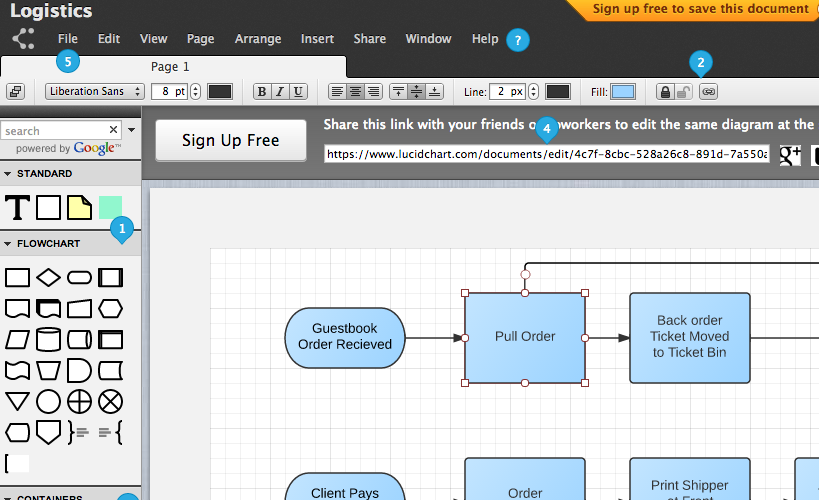
\includegraphics[width=160mm,keepaspectratio]{figures/lucid.png}\\

Lucidchart egy HTML5 és Javascript alapú diagramszerkesztő eszköz. \pdfcomment[icon=Note]{http://lifehacker.com/5112133/lucidchart-makes-stripped+down-flowcharts-for-free} 2008-ban lett béta verzióként elindítva.

 


%----------------------------------------------------------------------------
\section{Gliffy}
%----------------------------------------------------------------------------

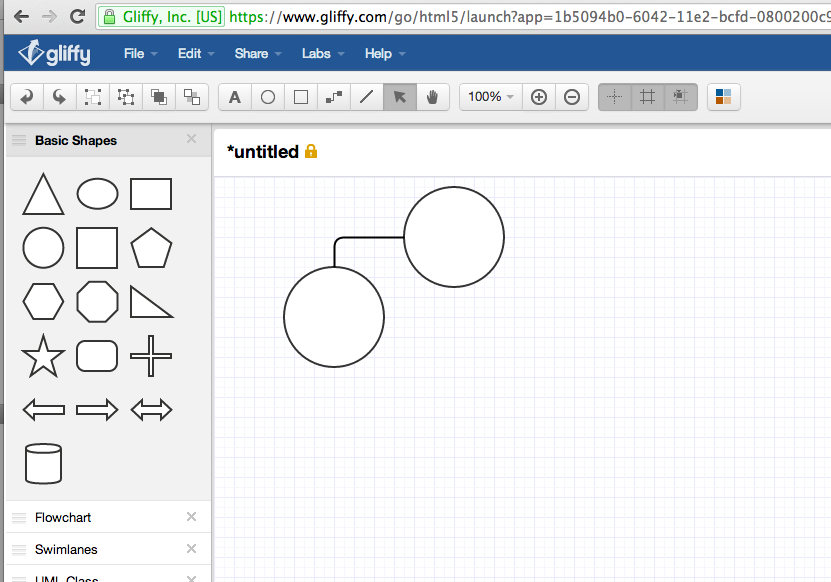
\includegraphics[width=160mm,keepaspectratio]{figures/gliffy.png}\\


Google Chrome plugin-ként offline üzemmódban is működik.


\section{Összefoglalás}


